\section{Reevaluation of theorem~\ref{eq:linear_gaussian_erm}}

To verify the theorem itself, we test it with a standard setting without the theorem results. This is reflected in Figure~\ref{fig:theorem_double_descent_fig}. The result is somewhat consistent with the theorem and its latter parameter error and prediction error results, however, this time, it correlates exactly as the prediction error instead. Additionally, peculiarity occurs in the non-double descent region, with much less volatility than in the prediction of the theorem. 

\RestyleAlgo{ruled}
\SetKwComment{Comment}{}{}
\begin{algorithm}[h!]
    \caption{Linear regression with Gaussian white noise, full control.}
    \KwData{$n,p,d,\sigma,r$, fixed range $[a,b]$, $u\in [0,1]$}
    \KwResult{Threefold error measure - MSE on parameters $p,d$, MSE on prediction $Y',Y$, and theoretical risks measure by prescription.}
    \Begin
    {\small
    $\mathrm{Randomizer}(\cdot)\gets\mathrm{PCG64}(n\leq 100)$\Comment*[r]{Randomizing pseudo-random engine}
    $\sigma\gets 0.5$, $d\gets 150$\Comment*[r]{Common presetting for parameters}
    $nl\gets\{12,\dots,280\}$\Comment*[r]{Common full-list $n$ count of datapoints}
    $p\gets 150$\Comment*[r]{Underparameterization to equal}
    $\mathbf{p}\gets \mathrm{range}(1,p)$\; $[a,b]\gets [-100,100]$\;
    $w_{c}\sim \mathrm{PCG64}.\mathrm{Uniform}([1,d],150)$\; $b_{c}\sim \mathrm{PCG64}.\mathrm{Uniform}([1,10])$\;
    $w_{p}\sim \mathrm{PCG64}.\mathrm{Uniform}([1,p],p)$\; $b_{p}\sim \mathrm{PCG64}.\mathrm{Uniform}([1,10])$\;
    $X\sim\mathrm{PCG64}.\mathrm{Uniform}(\mathrm{range}\gets[a,b],\mathrm{size}\gets[n,d])$\Comment*[r]{$n$ samples of $d$ dimensions.}
    $\mathrm{concept}(\cdot,\cdot,\cdot)\gets (d,w_{c},b_{c})$\;
    $Y \gets \mathrm{concept}(X, w_{c},b_{c})$\;
    $\sigma_{\mathrm{scaled}} \gets \sigma \cdot \mathbb{E}\left[\lvert Y\rvert\right]$\;
    $Y \gets Y + \mathrm{PCG64}.…\mathrm{Normal}\left(\mu\gets 0,\;\sigma\gets \sigma_{\mathrm{scaled}},\;\mathrm{size}\gets\lvert Y\rvert\right)$ \Comment*[r]{Noisy featuring}

    \For{$n\in nl$}{
        $w_{p}^{*}\gets\mathrm{PCG64}.\mathrm{Permutation}(d,p)$\;
        \For{$i\gets 1$ \KwTo $\lvert w_{p}\rvert$}{
            \If{$i\neq w^{*}_{p}$}{
                $w_{p}[i]\gets 0$, fixed zero point. 
            }
        }
        $\mathrm{model}(\cdot,\cdot,\cdot)\gets (d,w_{p},b_{p})$\;
        $Y\gets \mathrm{model}(X,w_{p},b_{p})$\;
        $\mathrm{approx}\gets \mathrm{LeastSquare}(\mathrm{model},Y',X,Y)$, fixed $w_{p}$.
    }
    $\mathrm{MSE}_{\mathrm{param}}(\cdot,\cdot,\cdot)\gets \mathrm{MSE}(Y,\{\mathrm{approx}\},\mathrm{model})$\;
    $\mathrm{MSE}_{\mathrm{pred}}(\cdot,\cdot)=\mathrm{MSE}(Y,Y')$
    $\hat{R}_{\mathrm{Thm}}=\mathrm{TR}(w_{c},\sigma,p,d,n)$\;
    }
    \Return{$\mathrm{MSE}_{\mathrm{param}}$, $\mathrm{MSE}_{\mathrm{pred}}$,$\hat{R}_{\mathrm{Thm}}$}
    \label{algo:algo_reg_lin_1}
\end{algorithm}

We use the Algorithm~\ref{algo:algo_reg_lin_1} for verification, including three modes of error measure, which will then be calculated accordingly. For gradient descent, we refer to another experiment. For such algorithm, we notice that the operational space of the model is $\mathbb{R}^{n}\to \mathbb{R}$. The masking of parameters then is not well-received, since the output space is far more skewed - single dimension resultant with no scaling difference because the model in question is supposed to be linear. Regarding such, it makes sense to realize that the model itself can still attain relatively stable error, because its feature compounds on the scaling parameters

To test the stability of the model, we run for a stable section of the permutations done on $p$. The result is outlined in \ref{fig:theorem_double_descent_fig}. Interestingly, while the interpolation threshold theorized being $p=n$ does not hold, the pattern of double descent without head descent still fundamentally exists, albeit in a much more constrained region, as can see from $n=12$ to $n=150$. The pattern from then onward follows a reduced trend, without the chaotic behaviours seen. The result is shown in Figure~\ref{fig:theorem_double_descent_fig4}.

\begin{figure}
    \centering
    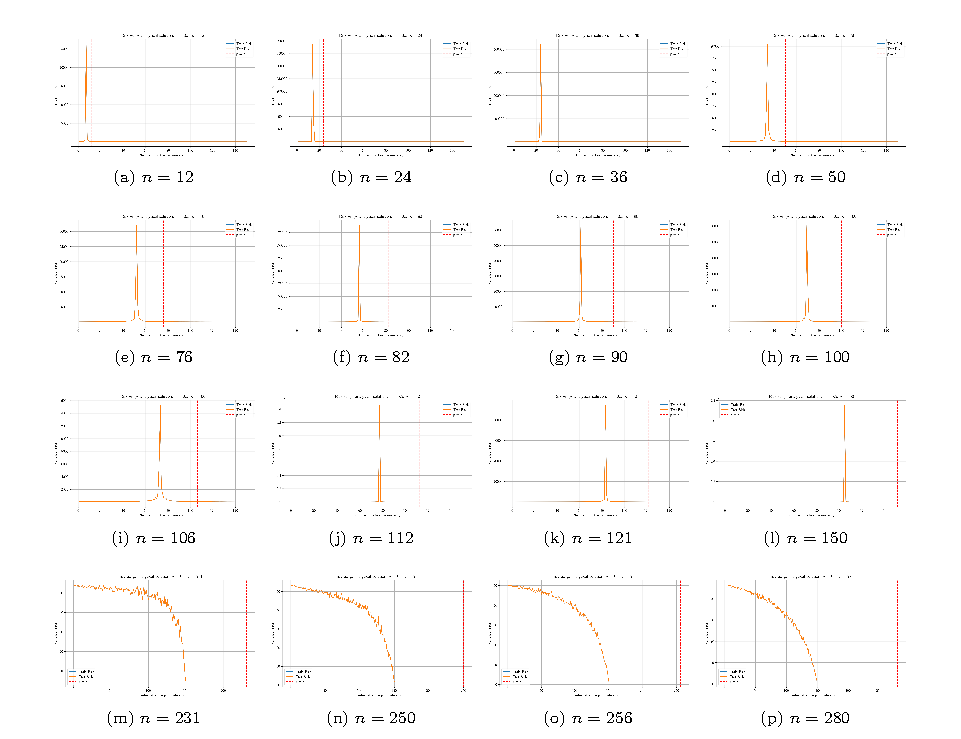
\includegraphics[width=0.6\textwidth]{pdf/theorem_4_verify.pdf}
    \caption{Risk curves for varying sample size $n$ (dimension $d=100$, noise $\sigma=0.5$). Double descent is determined in similar sequence, even though the interpolation theoretical $p=n$ is actually shifted over to the right from the actual interpolation observables, in parameterization. Afterward, correlation fails, and the theoretical $p$ is ineffective, similar to previous theorem-based test run. Sample set size range is $n\in\{12,24,36,50,76,82,90,100,106,112,121,150,231,250,256,280\}$. One additional remark is that the error landscape is relatively thin in either side, making it abnormal in comparison to actual bias-variance curvature.}
    \label{fig:theorem_double_descent_fig4}
\end{figure}

\subsection{Remark}

At least from this experiment, overall, results gathered using Theorem~\ref{thm:double_descent_lr} and variations of it suggests inconsistent results. The supposed interpolation threshold has different interpretation and indication in different scenario, including both parameter-wise error and prediction-only error measure. Furthermore, verification also shows inconsistency with the interpolation threshold, albeit given the fact that the margin of error from the highest peak to the interpolation point is consistent up to certain $n$. Breakdown of the result from theorem, as well as double descent behaviour starts with high $n$ counts, as well as interesting outlook of bias-variance reappearance for $p\sim 5000$, far more than what is tested in normal testing cases. Such result suggests further experiments to validate the observations, as well as statistical analysis of the entire system. 

Specifically, the interpretation of the result is not perfect. Under such setting, then for the concept of the same class, so $d=150$, any concept of $p>d$ would result in the metric taking zero value of the `truncated region' where $d$ is literally flat on the $d+1$ onward space. Hence, the error being added on top of such error measure is the component distance of $p$ to the flat sub $p-d$ space itself - which explains the curve going upward, as more and more risks are configured. Nevertheless, the amount of data provided, at least in terms of this model, does indeed have non-trivial effect on the model itself, and the least square solution of best fit which gives the potential minimal, hence the empirical best. Considering the results, we can see regions where the theorem `breaks' of its bias-variance pattern. Further experiment to verify such claim and reconfiguration is needed. Worryingly, in this particular case, there exists no saddle point that was theorized by bias-variance tradeoff, which must then be explained accordingly. Furthermore, we also notice the troublesome fact that this particular pattern works on \textit{same operational space} models, that is, linear models approximating linear models. This setting is fairly limited, and would not generalize well. However, we also do not know what kind of measure to take in such case. Conflicting notions and reports aid into the confusion of such topic more than can be normally observed, and the anomalous behaviours in some researches (for example, in \cite{shi2024homophilymodulatesdoubledescent}, we received that in GNN, there exists no trace of double descent) makes it even harder. As such, both the status of bias-variance being false, albeit in a given range only, and double descent in masking certain behaviours of the modelling process, have taken a mysterious stance in the modern machine learning community.

While discovering the double descent phenomena, it also exposes theoretical concepts that are not organized or formalized, portions of the theory and empirical observations that are within conflict of each others, issues with definitions, theorems, and interpretation of them. Those problems would then ultimately hinder further research in such direction, as well as broader theoretical requirement of the theory of machine learning, and specifically to a larger and more complex system of deep learning. 

\section{Observing gradient descent decomposition}

While the interpretation of what the bias-variance tradeoff, the usual training-versus-test curve, and statistical learning consideration, another interesting aspect to consider (as well for double descent), is how bias-variance decomposition acts on gradient descent and its components. This claim is perhaps reinforced by the work of \cite{adlam2020understandingdoubledescentrequires} which indicates that different bias-variance decompositions effects differently on the total system mechanism. 

\begin{figure}
    \centering
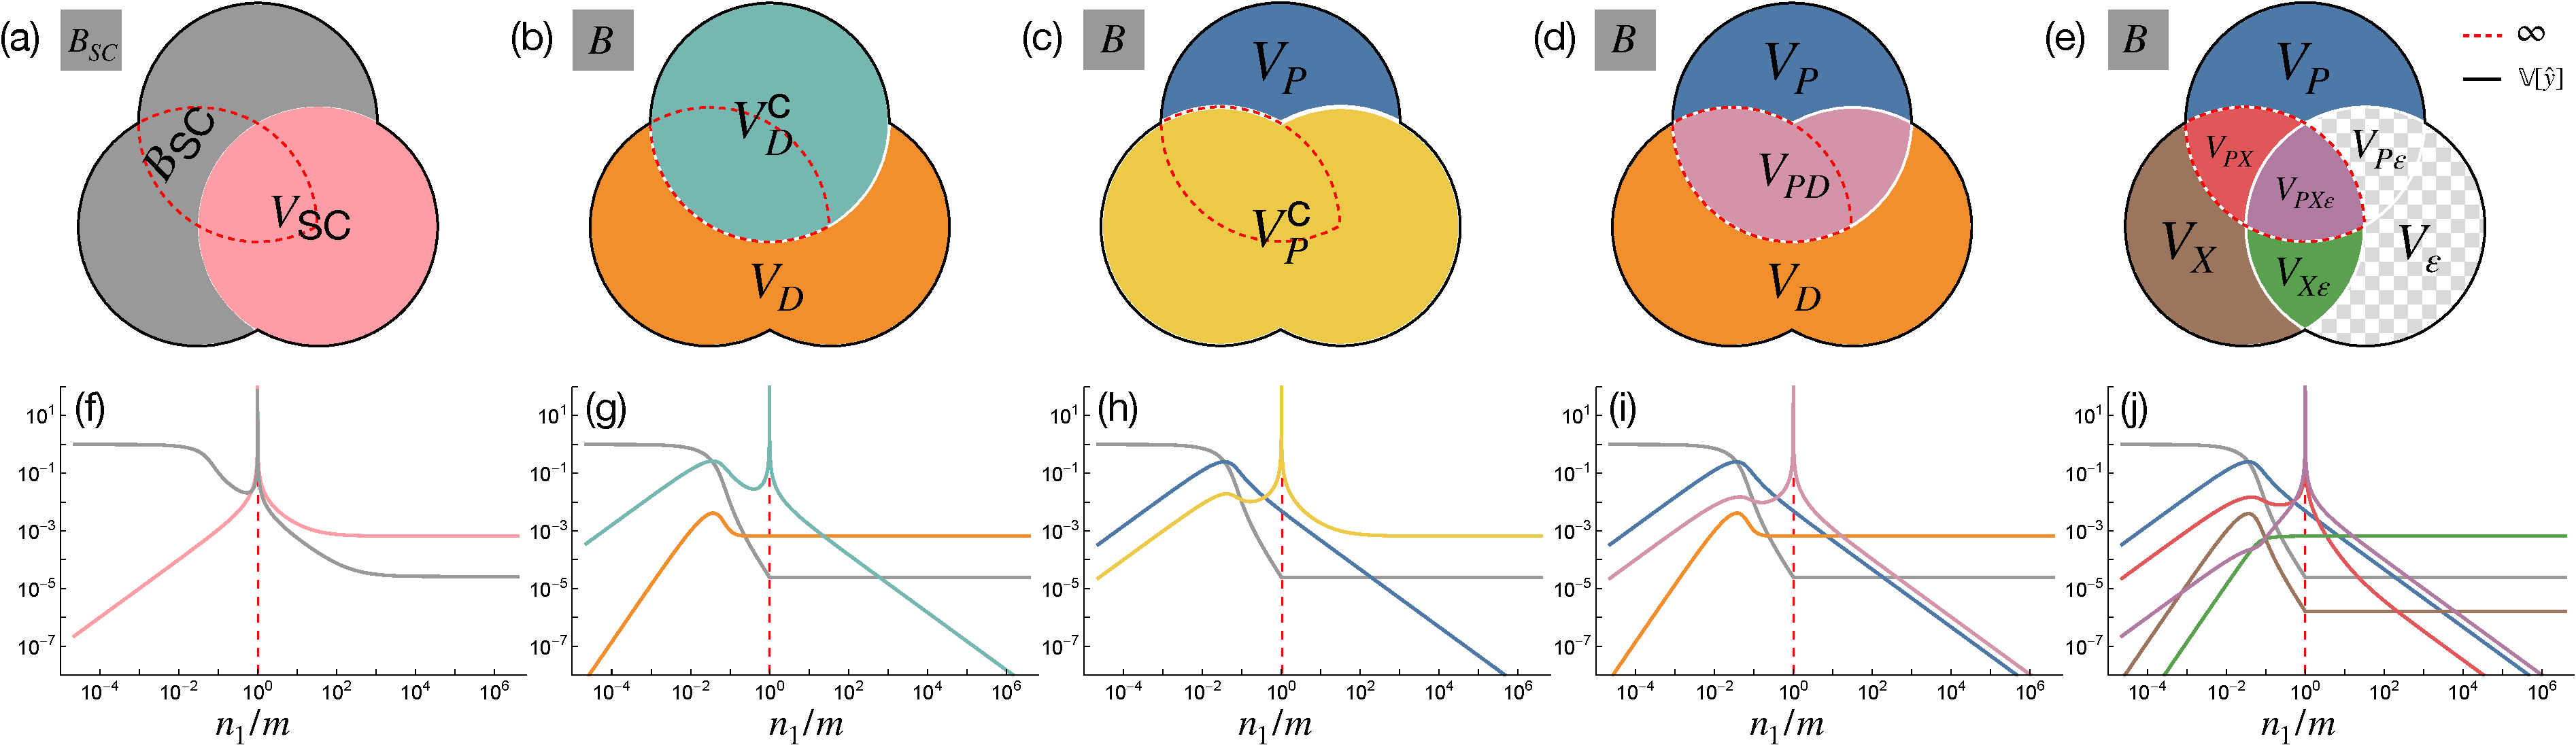
\includegraphics[width=\linewidth]{pdf/VennFig2.pdf}
\caption{(\textbf{a-e) The different bias-variance decompositions.} (f-j) Corresponding theoretical predictions for $\gamma =0$, $\phi=1/16$ and $\fs = \tanh$ with $\text{SNR} = 100$ as the model capacity varies across the interpolation threshold (dashed red). (a,f) The semi-classical decomposition of~\cite{hastie2019surprises,mei2019generalization} has a nonmonotonic and divergent bias term, conflicting with standard definitions of the bias. (b,g) The decomposition of~\cite{neal2018modern} utilizing the law of total variance interprets the diverging term $V_D^\textsc{c}$ as ``variance due to optimization''. (c,h) An alternative application of the law of total variance suggests the opposite, \emph{i.e.} the diverging term $V_P^\textsc{c}$ comes from ``variance due to sampling''. (d,i) A bivariate symmetric decomposition of the variance resolves this ambiguity and shows that the diverging term is actually $V_{PD}$, \emph{i.e.} ``the variance explained by the parameters and data together beyond what they explain individually.'' (e,j) A trivariate symmetric decomposition reveals that the divergence comes from two terms, $V_{PX}$ and $V_{PX\bfe}$ (outlined in dashed red), and shows that label noise exacerbates but does not cause double descent. Since $V_\e=V_{P\e}=0$, they are not shown in (j). Taken from \cite{adlam2020understandingdoubledescentrequires}}
\label{fig:venn_variance}
\end{figure}

The main term of a gradient descent algorithm is the gradient of the loss function $\mathcal{L}(h(x),y)$. For the hypothesis $h$, the number of instances supplied denoted by $k$ has three main cases: $k=1$ for stochastic descent, $k\in (1,m)$ for batch gradient descent, and $k=m$ for standard gradient descent, for a given space of $m$ samples. The gradient in such case is calculated using the empirical risk on $m$ size, that is: 
\begin{equation}
    \mathcal{L}_{k}(h(x),y) = \hat{R}_{S[k]}(h) = \frac{1}{k} \sum^{k}_{i=1} \ell(h(x_{i}),y_{i})
\end{equation}
We use the classical bias-variance tradeoff at first. Since the gradient is a linear operator, we have: 
\begin{equation}
    \begin{split}
        \nabla_{k}(\mathcal{L}) &= \nabla_{k}\left(\pa{\E\hat{y}(\bfx) - \E y(\bfx)}^2 + \V\qa{\hat{y}(\bfx)} + \V\q{y(\bfx)}\right)\\
        & = \nabla_{k}\left( \E\left[\hat{y}(\bfx)\right] - \E\left[y(\bfx)\right] \right)^2 + \nabla_{k}\V\left[\hat{y}(\bfx)\right] + \nabla_{k}\V\left[y(\bfx)\right] \\
        & = \nabla_{k}\left( \E\left[\hat{y}(\bfx)\right] - \E\left[y(\bfx)\right] \right)^2 + \nabla_{k}\V\left[y(\bfx)\right]
    \end{split}
\end{equation}
This effectively decompose the gradient into three parts that influence the overall gradient calculation. Because $\nabla_{k}\V\left[y(\bfx)\right]$ calculates the gradient of irreducible error, which is supposed to be constant of the sample space, it is then equal $0$. Suppose a sample $\mathbf{x}_{k}$ of size $km$, of partition $k$. Hence, we have gradient descent based on $k$th run over the entire dataset, permuted. Then, the loss function calculates in the form 
\begin{equation}
  \begin{split}
    \nabla_{k,n}(\mathcal{L}) &= \nabla_{k,n}\left[ \frac{1}{n}\sum_{i\leq n} \hat{y}(x_{kn+i})  - \frac{1}{n}\sum_{i\leq n} y(x_{kn+i}) \right]^{2} \\
    &+ \nabla_{k,n} \left[ \frac{1}{n}\sum_{i=1}^n y(x_i)^2 - \left( \frac{1}{n}\sum_{i=1}^n y(x_i) \right)^2 \right]
  \end{split}
\end{equation}
The indices is now changed to $(k,n)$ for $m/k=n$ as the $i$th partitioned, ordered run, thereby $kn+i$ runs for the index. If we assume a simplified structure $\theta_{t}$ of parameters $y(x_{i})$ depends on, we can reduce it further.  
\begin{equation}
\begin{split}
    &\nabla_{k,n}(\mathcal{L}) \\
&= 2\left(
      \frac{1}{n}\sum_{i=1}^{n}\hat{y}(x_{kn+i})
      - \frac{1}{n}\sum_{i=1}^{n}y(x_{kn+i})
   \right) \\
   & 
   \times \left(
      \frac{1}{n}\sum_{i=1}^{n}\nabla_k \hat{y}(x_{kn+i})
      - \frac{1}{n}\sum_{i=1}^{n}\nabla_k y(x_{kn+i})
   \right) \nonumber\\ %[0.3em]
&
   + \frac{2}{n}\sum_{i=1}^{n} y(x_i)\,\nabla_k y(x_i)
   - \frac{2}{n^2}
     \left( \sum_{i=1}^{n} y(x_i) \right)
     \left( \sum_{i=1}^{n} \nabla_k y(x_i) \right) \\
&= 2\Big[
      \big( \mathbb{E}_n[\hat{Y}] - \mathbb{E}_n[Y] \big)
      \big( \mathbb{E}_n[\hat{G}_k] - \mathbb{E}_n[G_k] \big) \\
      & \quad \quad 
      + \mathbb{E}_n[Y G_k]
      - \mathbb{E}_n[Y]\,\mathbb{E}_n[G_k]
   \Big] \\ 
& = 2\Big[
      \big( \mathbb{E}_n[\hat{Y}] - \mathbb{E}_n[Y] \big)
      \big( \mathbb{E}_n[\nabla_k \hat{Y}] - \mathbb{E}_n[\nabla_k Y] \big)\\
& \quad \quad + \mathrm{Cov}_n(Y,\nabla_k Y) \Big] \\ 
& = 2 \big( \mathbb{E}_n[\hat{Y}] - \mathbb{E}_n[Y] \big) \big( \mathbb{E}_n[\nabla_k \hat{Y}] - \mathbb{E}_n[\nabla_k Y] \big) \\
& \quad \quad + 2\,\mathrm{Cov}_n(Y,\nabla_k Y)
\end{split}
\end{equation}

for the expectation over $Z_{i}$, and covariance, 
\begin{equation}
    \mathbb{E}_n[Z] = \frac{1}{n} \sum_{i=1}^n Z_i,
\quad
\mathrm{Cov}_n(U,V) = \mathbb{E}_n[UV] - \mathbb{E}_n[U] \,\mathbb{E}_n[V].
\end{equation}
Here, we can see two terms multiplication, for the first one being the correlation between the expected error $\mathbb{E}_n[\hat{Y}] - \mathbb{E}_n[Y]$ and the gradient $\mathbb{E}_n[\nabla_k \hat{Y}] - \mathbb{E}_n[\nabla_k Y]$. This measures the correlation between the expected error, and the gradient measure. The second term is exactly the empirical covariance between the target $Y$ and the true gradient component. Since we are taking a fixed concept case, we can simply disregard the truth gradient hence $\mathbb{E}_n[\nabla_k Y]$, for which the term is reduced to $2\left( \mathbb{E}_n[\hat{Y}] - \mathbb{E}_n[Y] \right) \left( \mathbb{E}_n[\nabla_k \hat{Y}] \right)$. Under this same assumption applied to the covariance term, we obtain
\begin{equation}
    \begin{split}
        \nabla_{k,n}(\mathcal{L}) 
&= \frac{2}{n}\sum_{i=1}^n \big(\hat Y_i - Y_i\big)\,\partial_k \hat Y_i \\
&= 2\left(
   \left( \mathbb{E}_n[\hat{Y}] - \mathbb{E}_n[Y] \right)
   \mathbb{E}_n[\nabla_k \hat{Y}]
\right)
    \end{split}
\end{equation}
Looking into some particular algebraic representation, we can write this simply as
\begin{align}
    \nabla_{k,n}\mathcal{L}
    &= 2\,\mathbb{E}_n\!\left[(\hat Y - Y)\,\nabla_k \hat Y\right] \\
    &= 2\Bigg(
    \underset{\left[\mathbb{B}(\hat{Y},Y)\right]^{1/2}}{\underbrace{\bigl(\mathbb{E}_n[\hat Y] - \mathbb{E}_n[Y]\bigr)}}\,\mathbb{E}_n[\nabla_k \hat Y]\\
    &+ \underset{\mathrm{Cov}_n(\hat Y,\,\nabla_k \hat Y)}{\underbrace{\mathbb{E}_n[\hat Y\,\nabla_k \hat Y] - \mathbb{E}_n[\hat Y]\,\mathbb{E}_n[\nabla_k \hat Y]}}
     \\
    & \quad -\underset{\mathrm{Cov}_n(Y,\,\nabla_k \hat Y)}{\underbrace{\mathbb{E}_n[Y\,\nabla_k \hat Y] - \mathbb{E}_n[Y]\,\mathbb{E}_n[\nabla_k \hat Y]}}
    \Bigg)
\end{align}

The first term can be attributed to self-correct of bias-error gradient correlation, while the two covariance term suggests correlation between model randomness and its gradient, and the last one deal with the truth-gradient correlation. What those gradients mean will have to be tested in some preliminary models. Generally, we should not expect the result to be quite effective. Similar decomposition can be conducted for the other decomposition, as suggested, however, the gradient effect is particularly interesting, and will have to be resolved. 

\section{Details of supervised learning structure}

In a typical machine learning setting, we obtain assume the following figure~\ref{fig:PhaseDiagram}. This includes the ground, input space (the setting of which the observations are observed), the concept $c\in\mathcal{C}$, the hypothesis $c\in \mathcal{H}$, and a supervisor $\nabla$ that `correct' the behaviours of the hypothesis to match with $c$. This is called a supervised learning setting, in which the learning part is governed by the supervisor and the observations from the concept.

\begin{figure}
    \centering
    \captionsetup{font=small}
    \resizebox{0.7\textwidth}{!}{%
    \begin{circuitikz}
    \tikzstyle{every node}=[font=\normalsize]
    \draw  (6.25,20.5) rectangle  node {\normalsize $\mathbf{X}$} (7.5,15.5);
    \draw [->, >=Stealth, dashed] (7.5,19.25) -- (10,19.25)node[pos=0.5, fill=white]{$x\in\mathbf{X}$};
    \draw  (10,17.25) rectangle  node {\normalsize $h\in\mathcal{H}$} (13.75,16.25);
    \draw  (10,19.75) rectangle  node {\normalsize $c\in\mathcal{C}$} (13.75,18.75);
    \draw  (16.25,20.5) rectangle  node {\normalsize $\nabla(\cdot)$} (17.5,15.5);
    \draw [->, >=Stealth] (13.75,19.25) -- (16.25,19.25)node[pos=0.5, fill=white]{$c(X)$};
    \draw [->, >=Stealth] (13.75,16.75) -- (16.25,16.75)node[pos=0.5, fill=white]{$h(X)$};
    \draw [->, >=Stealth, dashed] (16.25,16.75) .. controls (14.75,15.25) and (12.25,15.25) .. (12,16.25)node[pos=0.5, fill=white]{$\mathsf{Update}$};
    \draw [->, >=Stealth, dashed] (7.5,16.75) -- (10,16.75)node[pos=0.5, fill=white]{$x$$\in$$\mathbf{X}$};
    %\draw [dashed] (5.5,21) rectangle  (9,15) node[below=2pt, pos=0.5] {\normalsize $I$};
    %\draw [dashed] (9.5,21) rectangle  (14.25,15) node[below=2pt, pos=0.5] {\normalsize $II$};
    %\draw [dashed] (14.75,21) rectangle  (18.5,15) node[below=2pt, pos=0.5] {\normalsize $III$};
    \draw [dashed] (5.5,21) rectangle (9,15);
    \node at ($(5.5,15)!0.5!(9,15) + (0,-7pt)$) {\normalsize $\mathrm{I}$};
    
    \draw [dashed] (9.5,21) rectangle (14.25,15);
    \node at ($(9.5,15)!0.5!(14.25,15) + (0,-7pt)$) {\normalsize $\mathrm{II}$};
    
    \draw [dashed] (14.75,21) rectangle (18.5,15);
    \node at ($(14.75,15)!0.5!(18.5,15) + (0,-7pt)$) {\normalsize $\mathrm{III}$};
    \end{circuitikz}
    }%
    \caption{An illustration of the (supervised) statistical process. Phase III contains two parts: First is the evaluation $\nabla(h,c)$ according to the data $\mathcal{D}$, and second is the $\mathsf{Update}$ process to re-align $c$ to the actual target.}
    \label{fig:PhaseDiagram}
\end{figure}
\subsection*{Phase 1.}
Begin with the construction and initialization of the feature space $\mathcal{X}^{\infty}$. By the assumption of a probabilistic process, $\mathcal{X}_{m}$ or simply $\mathcal{X}$ representing the dataset is assumed to be sampled, or appeared from the distribution $\mathcal{D}(p,\cdot)$ for $p$ an arbitrary probabilistic system. 

The \textit{ground space}, or in literature generally called \textbf{feature space}, is created. This results in the first component of the tuple $D$, being $\mathcal{X}\subseteq \mathbb{R}^{m\times k}$, where $\lvert \mathcal{X} \rvert=m$, but $size(x)=k$, for $x\in\mathcal{X}$. We assume there exists the random variable $x$ of a given distribution $\mathcal{D}$, such that the set $\mathcal{X}\sim \mathcal{D}$ of all observation is given by an underlying distribution. A well-known assumption in this case is that $x\in\mathcal{X}$ has no dependent components. That is, for example, there does not exist any function $\psi_{x}: \{ x_{i} \}\to \{ x_{j} \}$, for $i\neq j$. (Thought, this only helps in Bayesian priori analysis). Furthermore, by specifying that $\mathcal{X}$ belongs to a specific distribution, we argue of the assumption that $x\in\mathcal{X}$ is \textit{independently and identically distributed} (i.i.d.), that is, for a given random sampling interpretation $S\subset\mathcal{X}\sim \mathcal{D}$, all data is sampled with the events space governed by the distribution $\mathcal{D}$ for every instance, and the existence of $x_{i}$ to $x_{j}$ for $i\neq j$ is none. 

The \textbf{role} of the distribution configuration is important. If $\mathcal{D}$ is uniform, that is, $D\sim \mathcal{U}(a,b)$, then we can disregard the aspect of $\mathcal{X}$ with random variables. For $[a,b]$ to be $(-\infty,+\infty)$, the problem changed to a \textit{regression problem}. If $\mathcal{D}$ is some other distribution function, then the problem of \textit{representative data} and \textit{population size} becomes apparent, which requires statistical analysis to be taken into consideration. 
\subsection*{Phase 2.}
For the constructed feature space $\mathcal{X}$, let $EX(c,\mathcal{D})$ be a procedure (or \textit{oracle}) acting on $\mathcal{C}$ and $\mathcal{X}$ to output $\langle x,c(x)\rangle$. The hypothesis then contains a similar procedure $EX_{\mathcal{H}}(h,\mathcal{D})$, such that to output $\langle x,h(x)\rangle$. We call this the \textit{inference phase}. 
    
The feature space $\mathcal{X}$ is provided to $h$. We assume $c$ is processed of the same process, resulted in $\mathcal{Y}_{c}$. Then, $h(\mathcal{X})$ outputs the set of hypothesis' target $\mathcal{Y}_{h}$. Thereby, we are approximating the \textit{process} $c$ itself. We can approach this in two main ways\footnote{Note that, in some aspect, this is similar to the usage of mathematical simulation of certain dynamical system, or \textit{any} system that has certain patterns or relations observable.}: either \textit{deterministic} or \textit{probabilistic}\footnote{The model itself can be entirely deterministic, while the learning process is not. in fact, one of the very first assumption and axiomatic view of the learning problem is that learning occurs in a \textit{probabilistic setting}.}. We define such as followed. 
For the constructed feature space $\mathcal{X}$, let $EX(c,\mathcal{D})$ be a procedure (or \textit{orcale}) acting on $\mathcal{C}$ and $\mathcal{X}$ to output $\langle x,c(x)\rangle$. The hypothesis then contains a similar procedure $EX_{\mathcal{H}}(h,\mathcal{D})$, such that to output $\langle x,h(x)\rangle$. We call this the \textit{inference phase}. 
    

\begin{definition}[Deterministic - \textit{discriminative modelling}]
    A \textbf{deterministic model} $h_{d}$ assumes its internal space as followed. For any $h\in\mathcal{H}_{d}$ of deterministic model, $h$ is characterized by the mapping $h_{d}:\mathcal{X}\to \mathcal{Y}_{h}$, such that $h\in C^{n}$ of $n$-differential space. 
\end{definition}

Similarly, if the interpretation of the model is \textit{probabilistic}, we have the following definition of probabilistic-based model. 
\begin{definition}[Probabilistic - \textit{generative modelling}]
    A \textbf{probabilistic model} $h_{p}$ assumes its internal space as followed. For any $h\in\mathcal{H}_{p}$ of all probabilistic hypothesis, $h$ is characterized by the probability distribution $\Gamma(p_{X}(X))$, where $\Gamma$ is the discrete decision process outside the probabilistic interpretation. \footnote{The discrete decision process $\Gamma$ is very simple to argue. For example, given a Naive Bayes model with $p(C_{k}\mid D[i])$ of the dataset, the probability distribution is regarded as the argument $$Y^{*}=\underset{c_{k}\in C}{\mathrm{arg\:max}}\:P_{\theta}(c_{k}\mid x)=\underset{c_{k}\in C}{\mathrm{arg\:max}}P_{\theta}(x\mid c_{k})\cdot P(c_{k})$$}
\end{definition}
Notice that the process and the learning setting is probabilistic, however, the interpretation of the hypothesis $h$ can be either deterministic or probabilistic, or anything else. This puts the flexibility into the setting of the model, and permits us to consider various representation of the model structure. Furthermore, the hypothesis for the learning process is evaluated relative to the same probabilistic setting, in which the training takes place, and we allow hypotheses that are only approximation of the target concept \cite{10.5555/2930837,10.5555/200548}. 

The similarity between both of the two general types is that the model is characterized by their \textbf{parameters}, both \textbf{model-specific parameters} and \textbf{hyperparameters}. 
\subsection*{Phase 3.}
There exists an evaluator (or \textit{supervisor}) $\nabla (h,c)$ that evaluates specific \textit{loss framework} $\ell\{h(x),c(x)\}$ based on available information, and a \textit{update modifier} $U(\ell,\mathcal{A})$ of certain objective to algorithm $\mathcal{A}$. 
    
    In this step of the procedural setting, the \textit{supervisor} includes a loss function, $\ell$, which takes discrete arguments, and `binarily' evaluate the discrete result between $h$ and $c$. This loss function is supposed to have a global minimum, or at least a certain region of minimal approximation. We have the following definition. 

    \begin{definition}[Loss function]
        A loss function is a non-negative function $\ell :\mathcal{Y}\times\mathcal{Y}\to [0,+\infty)$. 
    \end{definition}
    
    In general, the following is supposed of the loss function: 
    \begin{conjecture}[Loss function convexity]
    For any supervisor $\nabla$ of a learner framework $\mathcal{L}(\mathcal{H},\mathcal{A})$, the loss function $\ell$ is assumed to be a $p$-converging function, or as a convex function. That is, for $\ell: \mathbb{R}^{n}\to \mathbb{R}$, then $\ell$ is convex on its domain, or is locally convex on $[a,b]\subset \mathbb{R}^{n}$, if, for $x,y\in\mathbb{R}^{n}$ of such interval, and for $\lambda \in [0,1]$, it satisfies \begin{equation}
        f(\lambda x + (1-\lambda)y) \leq \lambda f(x) + (1-\lambda) f(y)
    \end{equation}
    \end{conjecture}
Under a single structure, that is, for example, a class of mapping $\mathbb{R}^{n}\to\mathbb{R}$, there can exist many loss functions to be considered. Take for example the setting of regression analysis. Then, $\ell$ can be either the absolute error, $\lvert h(x)-c(x)\rvert$, or the $L^{2}$ norm, $\lvert\lvert h(x), c(x)\rvert\rvert_{2}$. Different loss function provides different path and landscape, though they still share somewhat similar interpolation patterns, or either some might be subjected to, under the consideration of a loss landscape, local minima than others. Furthermore, the form and representation of loss functions is not discrete - but rather based of its interpretation and the supposition of the underlying notion required for the loss function to operate in. For example, if the setting is \textit{generative}, the loss function would take the form of a \textit{divergence measure} between two probability distribution. Notice however, that the action potential provided by the model in their operation dissapears, or rather, is not considered, when using the loss function. 

Using such loss function, for the case of no noises or interference uncertainty, if the goal is to minimize the empirical risk on such dataset, then we call this the method of \textit{empirical risk minimization}, or ERM. This is born out of the consideration that in practice, the oracle $EX(c,\mathcal{D})$, and the actual generalization error $R(h)$ is not obtainable. 
\section*{Appendix D - Bias-variance decomposition derivation in \cite{6797087}}

\begin{proof}
    We present the original derivation of bias-variance tradeoff and its analysis from \cite{6797087}. Geman's paper is, by his own word, concerned of \textit{parametric models}, i.e. hypothesis class without strong assumption of parameters defined, though the definition of bias-variance tradeoff afterward and its justification is made in the sense of parametric model. We partially clarify\footnote{Generally, there is no definite definition on what would be considered non-parametric. Though, an example might be drawn from the (vanilla) neural network and Gaussian Process Regression (GPR)} this with the following definition as customary. 

    \begin{definition}[Parameterization]
        A \textbf{parametric model} is one that can be parameterized by a finite number of parameters. In general, for a hypothesis class $\mathcal{H}$of all parametric hypothesis is then expressed as:
        \begin{equation}
            \mathcal{H} = \{f(x;\theta): \theta \in \Theta \subset \mathbb{R}^{d}\}
        \end{equation} where $\Theta$ is called the \textit{parameter space}. A \textbf{nonparametric model} is one which cannot be parameterized by a fix number of parameters.   
    \end{definition}
    Suppose of a training dataset $\mathcal{D}$ of $N$ 2-tuples $(\mathbf{x}_{i},y_{i})$, that is: \begin{equation}
        \mathcal{D} = \{(\mathbf{x}_{1},y_{1}),\dots,(\mathbf{x}_{N},y_{N})\} \quad \lvert \mathcal{D} \rvert = N, \mathbf{x}\in \mathbb{R}^{d}, y \in \mathbb{R}
    \end{equation}
    The regression problem is to construct a function $f(\mathbf{x})\to y$ based on $\mathcal{D}$, which is denoted $f(\mathbf{x};\mathcal{D})$ to show this dependency. Then, 
    \begin{equation}
        \begin{split}
            &\mathbb{E}\left[ (y-f(\mathbf{x};\mathcal{D}))^{2}\mid \mathbf{x},\mathcal{D}\right]\\ & = \mathbb{E}\Big[\big( (y-\mathbb{E}[y\mid \mathbf{x}]+ (\mathbb{E}[y\mid \mathbf{x}]-f(\mathbf{x};\mathcal{D}))) \big)^{2}\mid \mathbf{x},\mathcal{D}\Big]\\
            & = \begin{multlined}
                \mathbb{E} \Big[ (y- \mathbb{E}[y\mid \mathbf{x}])^{2}\mid \mathbf{x},\mathcal{D} \Big] + \Big(\mathbb{E}[y\mid \mathbf{x}-f(\mathbf{x};\mathcal{D})]\Big)^{2} \\ + 2\mathbb{E} \big[(y-\mathbb{E}[y\mid \mathbf{x}])\mid \mathbf{x},\mathcal{D}\big]\cdot \big(\mathbb{E}[y\mid \mathbf{x}]-f(\mathbf{x;\mathcal{D}})\big)^{2} 
            \end{multlined} \\
            & = \mathbb{E} \Big[(y-\mathbb{E}[y\mid \mathbf{x}])\mid \mathbf{x},\mathcal{D}\Big] + \big(\mathbb{E}[y\mid \mathbf{x}]-f(\mathbf{x};\mathcal{D})\big)^{2}\\
            & \geq \mathbb{E} \big[(y-\mathbb{E}[y\mid \mathbf{x}])^{2}\mid \mathbf{x},\mathcal{D}\big]
        \end{split}
    \end{equation}
    Hence, we decompose it to: 
    \begin{equation}
        \begin{split}
            &\mathbb{E} \left[((y-f(\mathbf{x};\mathcal{D})))^{2}\mid \mathbf{x}, \mathcal{D}\right] \\
            & \quad = \mathbb{E}\left[(y-\mathbb{E}[y\mid \mathbf{x}])^{2}\mid \mathbf{x},\mathcal{D}\right] + (f(\mathbf{x};\mathcal{D})-\mathbb{E}[y\mid \mathbf{x}])^{2}
        \end{split}
    \end{equation}
    Where $\mathbb{E}\left[(y-\mathbb{E}[y\mid \mathbf{x}])^{2}\mid \mathbf{x},\mathcal{D}\right]$ is regarded to be a relative constant of variance on $y$ given $\mathbf{x}$. Taking the expectation on $\mathcal{D}$, we gain: 
    \begin{equation}
        \begin{split}
            &\mathbb{E}_{\mathcal{D}} \Big\{ \mathbb{E} \left[((y-f(\mathbf{x};\mathcal{D})))^{2}\mid \mathbf{x}, \mathcal{D}\right]\Big\} \\
            & = \mathbb{E}_{\mathcal{D}} \Big\{\mathbb{E}\left[(y-\mathbb{E}[y\mid \mathbf{x}])^{2}\mid \mathbf{x},\mathcal{D}\right] + (f(\mathbf{x};\mathcal{D})-\mathbb{E}[y\mid \mathbf{x}])^{2}\Big\}\\
            & = \begin{multlined}
                \mathbb{E}_{\mathcal{D}} \Big\{ \mathbb{E}\left[(y-\mathbb{E}[y\mid \mathbf{x}])^{2}\mid \mathbf{x},\mathcal{D}\right]\Big\} \: + \\ \mathbb{E}_{\mathcal{D}} \Big\{ (f(\mathbf{x};\mathcal{D})-\mathbb{E}[y\mid \mathbf{x}])^{2}\Big\}
            \end{multlined}
        \end{split}
    \end{equation}
    The second term is of importance, and is further decomposed to: 
    \begin{equation}
        \begin{split}
            & \mathbb{E}_{\mathcal{D}} \Big\{ (f(\mathbf{x};\mathcal{D})-\mathbb{E}[y\mid \mathbf{x}])^{2}\Big\} \\ 
            & = \mathbb{E}_{\mathcal{D}} \Big\{ (f(\mathbf{x};\mathcal{D})- \mathbb{E}_{\mathcal{D}}[f(\mathbf{x};\mathcal{D})] + \mathbb{E}_{\mathcal{D}}[f(\mathbf{x};\mathcal{D})] -\mathbb{E}[y\mid \mathbf{x}])^{2}\Big\} \\
            & = \mathbb{E}_{\mathcal{D}} \Big[(f(\mathbf{x};\mathcal{D})-\mathbb{E}_{\mathcal{D}}[f(\mathbf{x};\mathcal{D})])^{2}\Big] \\
            &\quad + \mathbb{E}_{\mathcal{D}} \Big[ (\mathbb{E}_{\mathcal{D}} [f(\mathbf{x};\mathcal{D})] - \mathbb{E}[y\mid \mathbf{x}])^{2} \Big] \\
            &\quad \quad +2\mathbb{E}_{\mathcal{D}}\Big[f(\mathbf{x};\mathcal{D})-\mathbb{E}_{\mathcal{D}}[f(\mathbf{x};\mathcal{D})]\Big]\\
            &\quad \quad \cdot (\mathbb{E}_{\mathcal{D}}[f(\mathbf{x};\mathcal{D})]-\mathbb{E}[y\mid \mathbf{x}]) \\
            & = \underbrace{\left\{ \mathbb{E}_{\mathcal{D}}[f(x;\mathcal{D})] - \mathbb{E}[y\mid x] \right\}}_{\text{bias term}} \\
            &\quad + \underbrace{\mathbb{E}_{\mathcal{D}} \left\{(f(x;\mathcal{D})- \mathbb{E}_{\mathcal{D}}[f(x;\mathcal{D})])^{2}\right\}}_{\text{variance term}}
        \end{split}
    \end{equation}
    which yields the desired bias-variance tradeoff. 
\end{proof}

\section{Practical consideration}

While we have been talking in the learning setting pretty loosely on the side of the data itself, it is the data that gives us the problem setting. For example, if the data is a pair $(X,Y)$ of input output representation, then we know that our working space would be $\mathbb{R}^n \times \mathbb{R}^m$ or any of its subset, given the fact that data must be encoded into numerical representations, even in discrete or logical case (in such case, typically, $0-1$ pair is enough). In more complex and complicated setting, for example, on the structure of a graph and its embedded representation, it is much more difficult to see the \textit{form of dataset} to be, hence, also the working space. 

Another thing with data is the \textit{availability of the data} and the \textit{distribution of the data} also matters. In some cases, our data consists of only skewed or partitioned sections of the actual concept range, at least up to the observable criterion of the concept (some concept does not exist in certain range, at least in a numerical example, and some other reasons). In the other case, the availability of data, meaning the density of data, as well as added \textit{observational effect} also alters the learning setting, simply because learning theory relies on, at least from our glance, simple statistical, observational learning from observation space, without the added structures. An actual, practical concern however, lies in the range of \textbf{practical empirical-generalization} setting. 

\subsection{Observational space partitioning}

Previously, we established that at least in said formal setting, generalization errors cannot be known beforehand. Thereby, all of our operations, procedures, processes has to be conducted using the observed data, or the sample space $\mathcal{S}$. A solution to utilize that is to consider the generalization region as the region of \textit{new, unseen observations} that while still is of the same concept $c$, but it is indeed, unseen if the model is never provided of such instances. Hence, it prompts the utilization of limited resources by then to partition the sample space into various subspaces, that would be then fed into the learning process as observational space. This is simply called \textbf{sample set partitioning}. Denoted the number of partition (discrete) as $k$, then for $k=2$, then this is called the \textbf{train-test partition} (or dataset). This contains a dataset $\mathbf{x}_{1}$ and $\mathbf{x}_{2}$ of the same original sample set, such that $\mathbf{x}_{1}/\mathbf{x}_{2}\geq 1$ (one is bigger than another, usually). The ratio does indeed affect the overall running procedure, accordingly \footnote{If $k>3$ and above, we call it the $n$th partitioning. If we further consider the choice of observational spaces being provided, then if $k>3$, and subspaces are chosen randomly, it is called \textbf{cross-validating partition}. The effect of them are fairly well-understood, and we might as well refer to authoritative sources on such issue.}.



Based on the above conclusion, the empirical error and generalized error can be re-calculated to fit the general scheme. For $\lvert \mathcal{S}\rvert = m$ and partition $k+p=m$ for train and test partition respectively, 
\begin{align}
    &\hat{R}_{k}(h) = \frac{1}{k} \sum^{k}_{i=1} \ell\{h(x_{i}),c(x_{i})\},\\
    &\hat{R}_{p}(h_{\mathcal{A}}) = \frac{1}{k} \sum^{p}_{i=1} \ell\{h_{\mathcal{A}}(x_{i}),c(x_{i})\}
\end{align}
where $h_{\mathcal{A}}$ is the result from the learning algorithm (procedure), for $h^{*}\neq h_{\mathcal{A}}$. Then, the empirical learning seeks to optimize the first term, that is, for the objective 
\begin{equation}
    \underset{h\in \mathcal{H}}{\argmin}\: \hat{R}_{k}(h) = \underset{h\in \mathcal{H}}{\argmin}\:\frac{1}{k} \sum^{k}_{i=1} \ell\{h(x_{i}),c(x_{i})\}
\end{equation}

and the generalization learning as: 
\begin{equation}
    \begin{split}
        &\underset{h\in \mathcal{H}}{\argmin}\: \hat{R}_{p}(h_{\mathcal{A}}) \\
        & = \hat{R}_{k}(h_{\mathcal{A}}) + \underset{h\in \mathcal{H}}{\argmin}\:\hat{R}_{p}(h_{\mathcal{A}})\\
        & =  \underset{h\in \mathcal{H}}{\argmin}\: \left[\frac{1}{k} \sum^{k}_{i=1} \ell\{h_{\mathcal{A}}(x_{i}),c(x_{i})\} + \frac{1}{k} \sum^{p}_{i=1} \ell\{h_{\mathcal{A}}(x_{i}),c(x_{i})\}\right]\\
        & = \underset{h\in \mathcal{H}}{\argmin}\: \left[\epsilon + \frac{1}{k} \sum^{p}_{i=1} \ell\{h_{\mathcal{A}}(x_{i}),c(x_{i})\}\right]
    \end{split}
\end{equation}
By the definition order, the generalization error can only be calculated post-$\mathcal{A}$. Hence, we often called the empirical, or $\mathsf{ERM}$-generalizer case to be dynamic, and the solution for $\mathsf{ERM}$ is tested statically on generalization set. This partition of order of computation though, brings up the problem of updating factors and others contributing potential that will damage or diffuse the measure. 

For cross-validation and other randomize partition, the formulation requires more care in the notion by itself. The structural risk minimization scheme dilemma can be understood from the above consideration naturally. We have effectively defined the two proxies, \textbf{heuristic empirical risk} and \textbf{heuristic generalization risk}. 